% 7. 在有氧锻炼中人的耗氧能力y (ml/min•kg) 是衡量身体状况是重要指标,它可能与以下因素有关:年龄x1,体重x2 (kg),1500米跑用的时间x3 (min),静止时心速x4 (次/min),跑步后心速x5 (次/min)。对24名40至57岁的志愿者进行了测试,结果如表13.28。试建立耗氧能力y与诸因素之间的回归模型。
% 1)	若x1~x5中只许选择1个变量,最好的模型是什么?
% 2)	若x1~x5中只许选择2个变量,最好的模型是什么?
% 3)	若不限制变量个数,最好的模型是什么?你选择哪个作为最终模型,为什么?
% 4) 对最终模型观察残差,有无异常点,若有,剔除后如何。

\subsubsection{算法设计}

\paragraph{第(1)问:一元回归} 对于一元回归,首先应当分别画出$y$与$x_1,x_2,x_3,x_4,x_5$的散点图,初步观察它们的相关性,如\Cref{fig:ex7_scatter}。可以看出,$y$关于$x_3$的图像呈现出明显的负相关,关于$x_4$和$x_5$呈现出较弱的负相关。进一步,可对每个自变量分别进行$n$次多项式回归,即,
\begin{equation}
    y = \sum_{i=0}^n \beta_i x^i + \varepsilon
\end{equation}

其中,$\beta_i$为回归系数,$x$可取$x_1,x_2,x_3,x_4,x_5$中的任意一个。注意到5个散点图均不具有明显的高次关系,因此线性回归模型应当足够表达因变量与自变量的相关性,可简化建模为,
\begin{equation}
    y = \beta_0 + \beta_1 x + \varepsilon
\end{equation}

在MATLAB中,可通过\texttt{regress}命令进行线性回归,通过\texttt{polytool}命令进行多项式回归。

\begin{figure}[H]
    \centering
    \subfigure[$y$-$x_1$图像]{
        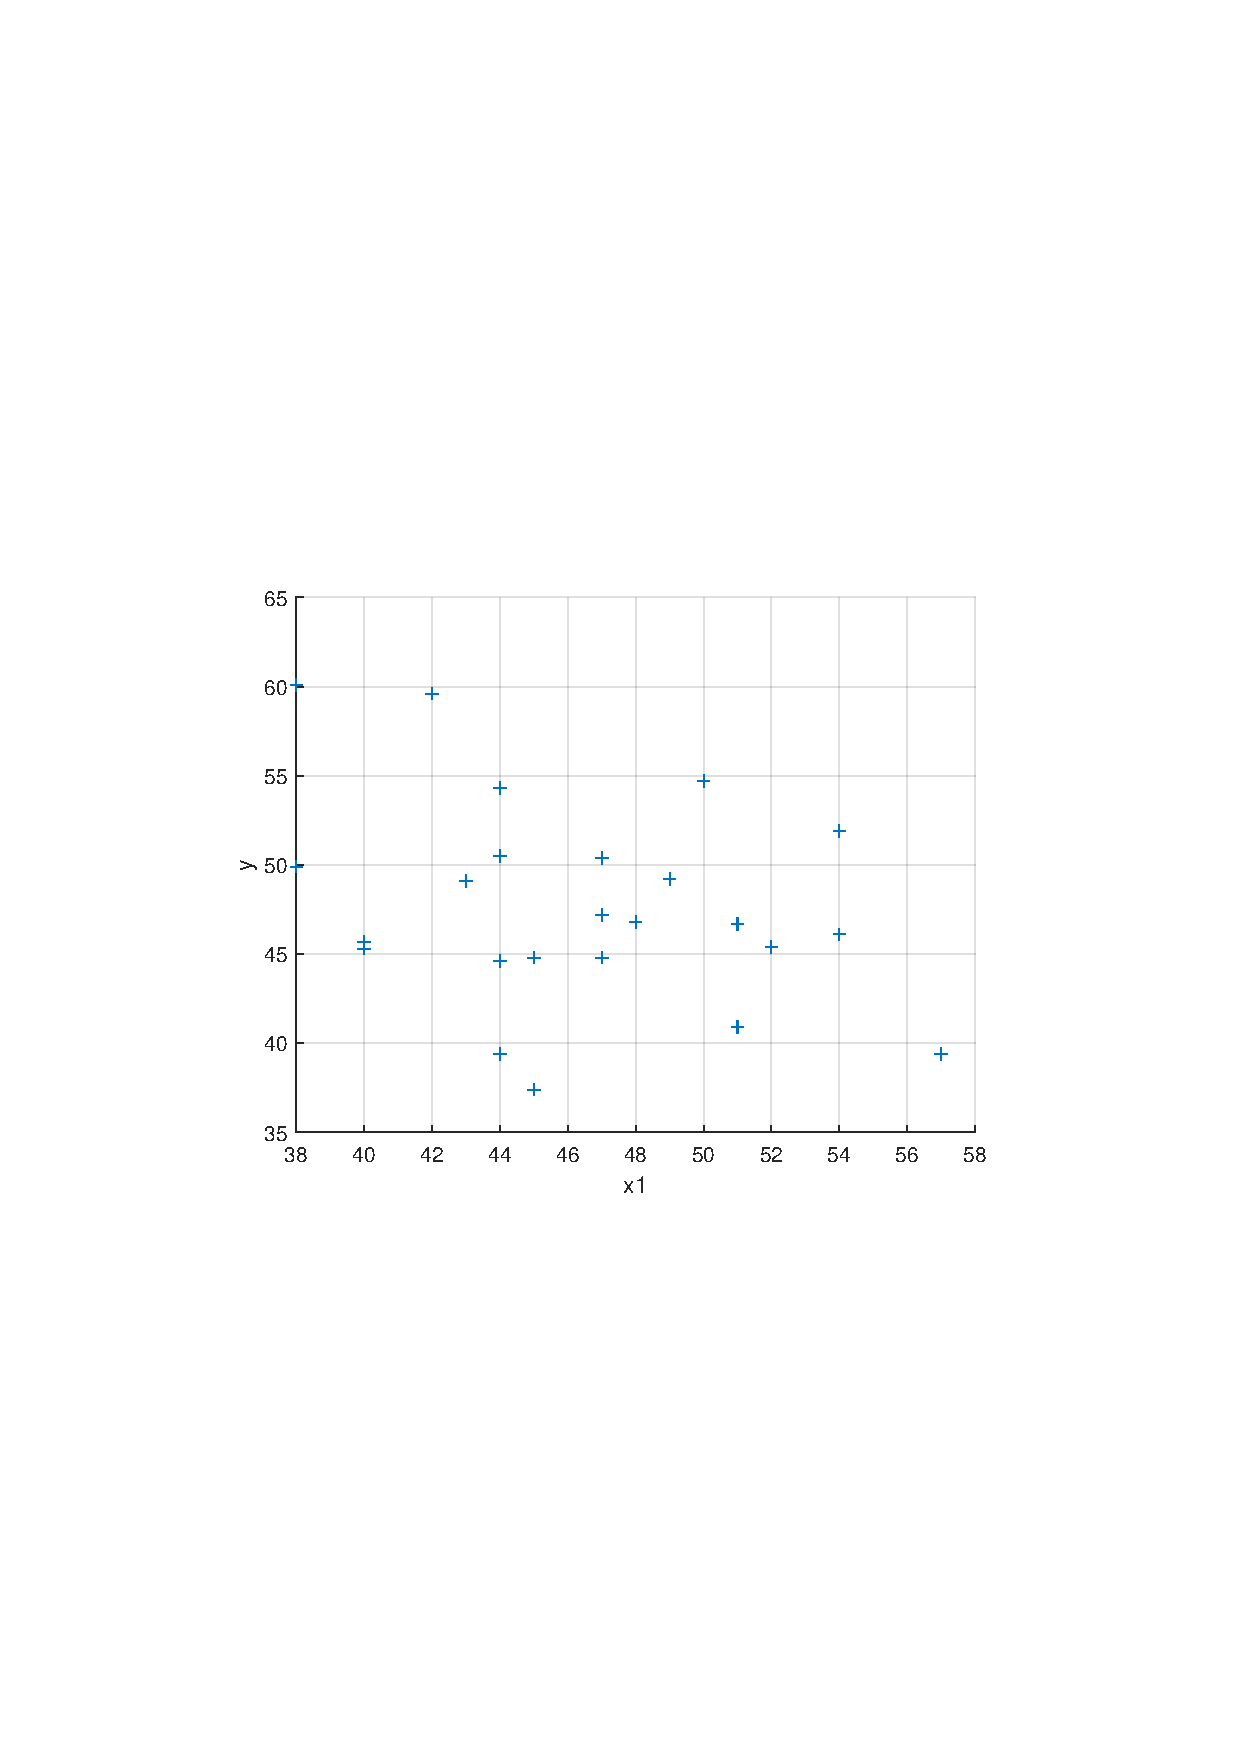
\includegraphics[width=0.3\textwidth,trim={3.09cm 9.295cm 3.09cm 9.295cm},clip]{fig/ex7_scatter_x1.pdf}
    }
    \subfigure[$y$-$x_2$图像]{
        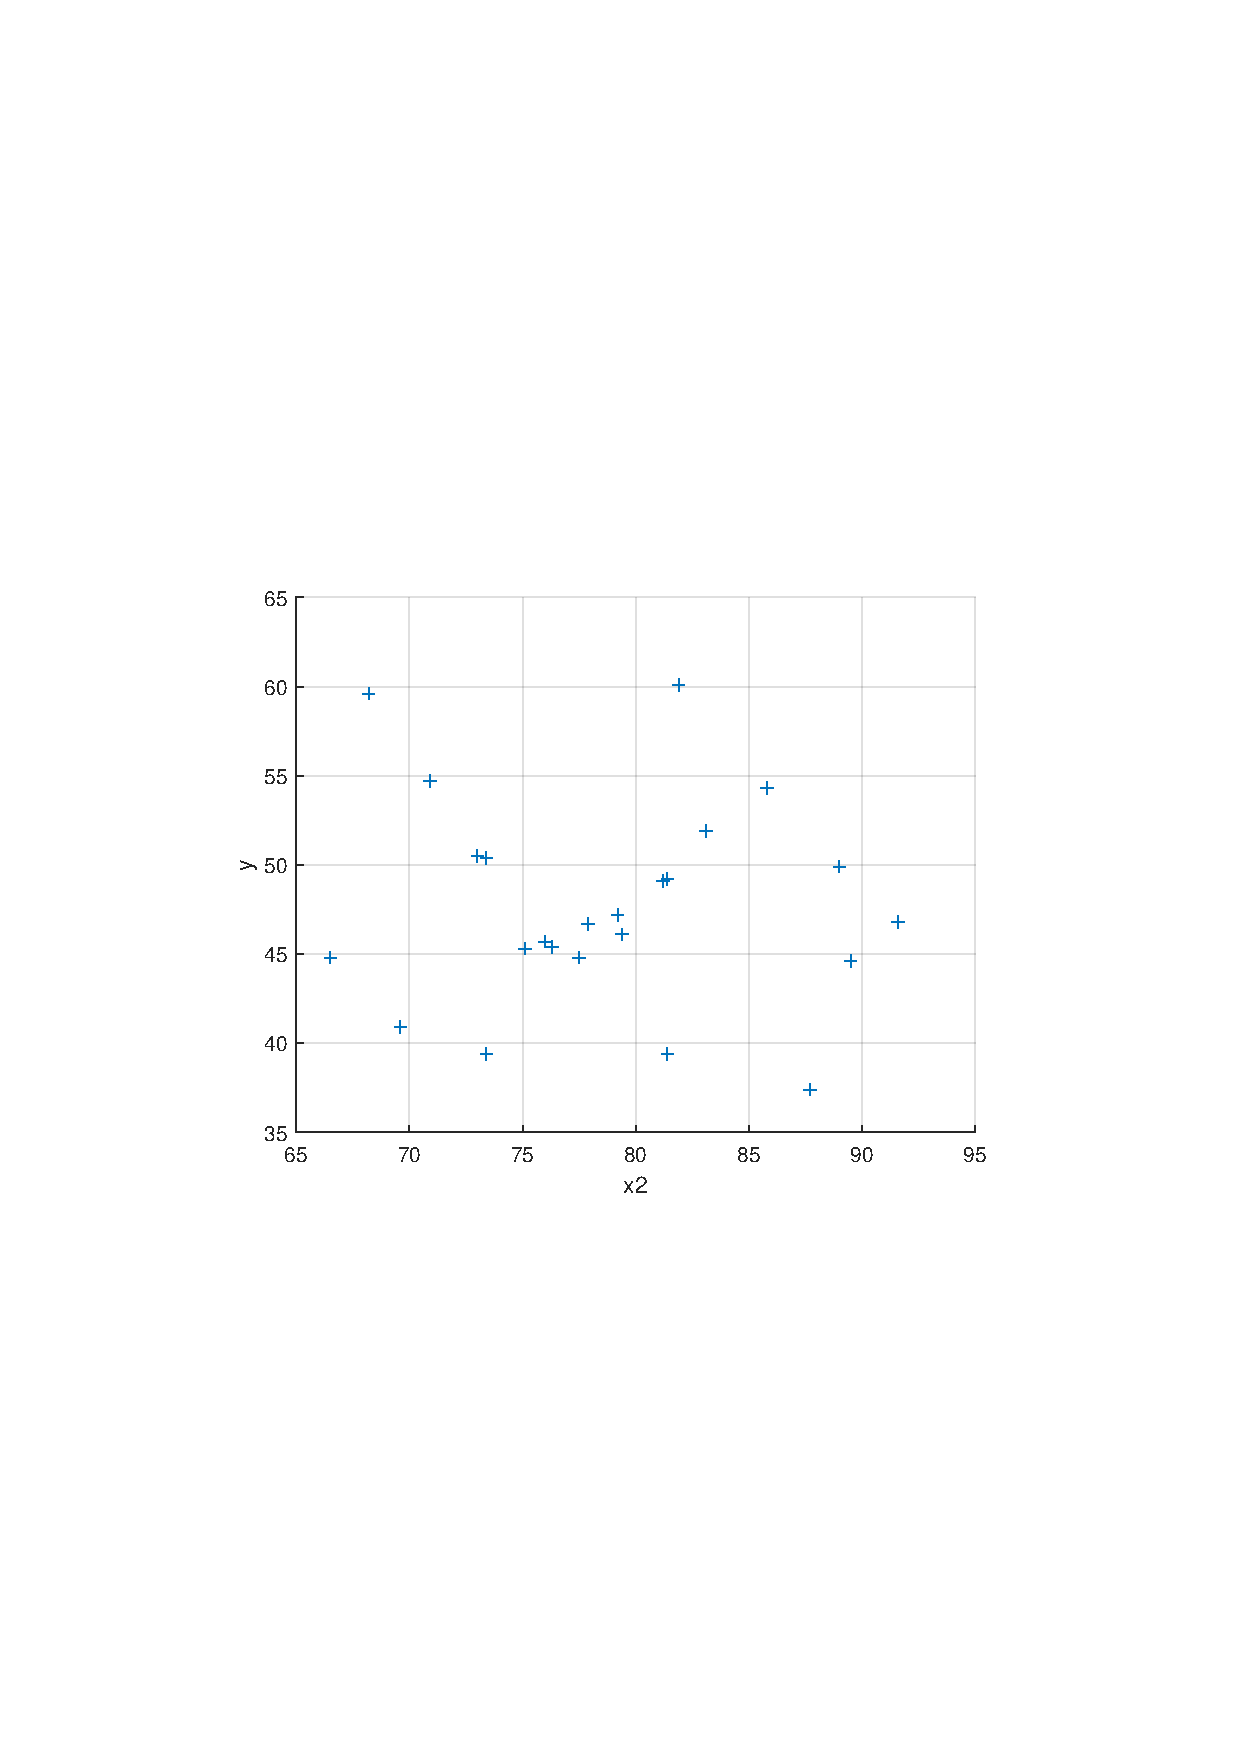
\includegraphics[width=0.3\textwidth,trim={3.09cm 9.295cm 3.09cm 9.295cm},clip]{fig/ex7_scatter_x2.pdf}
    }
    \subfigure[$y$-$x_3$图像]{
        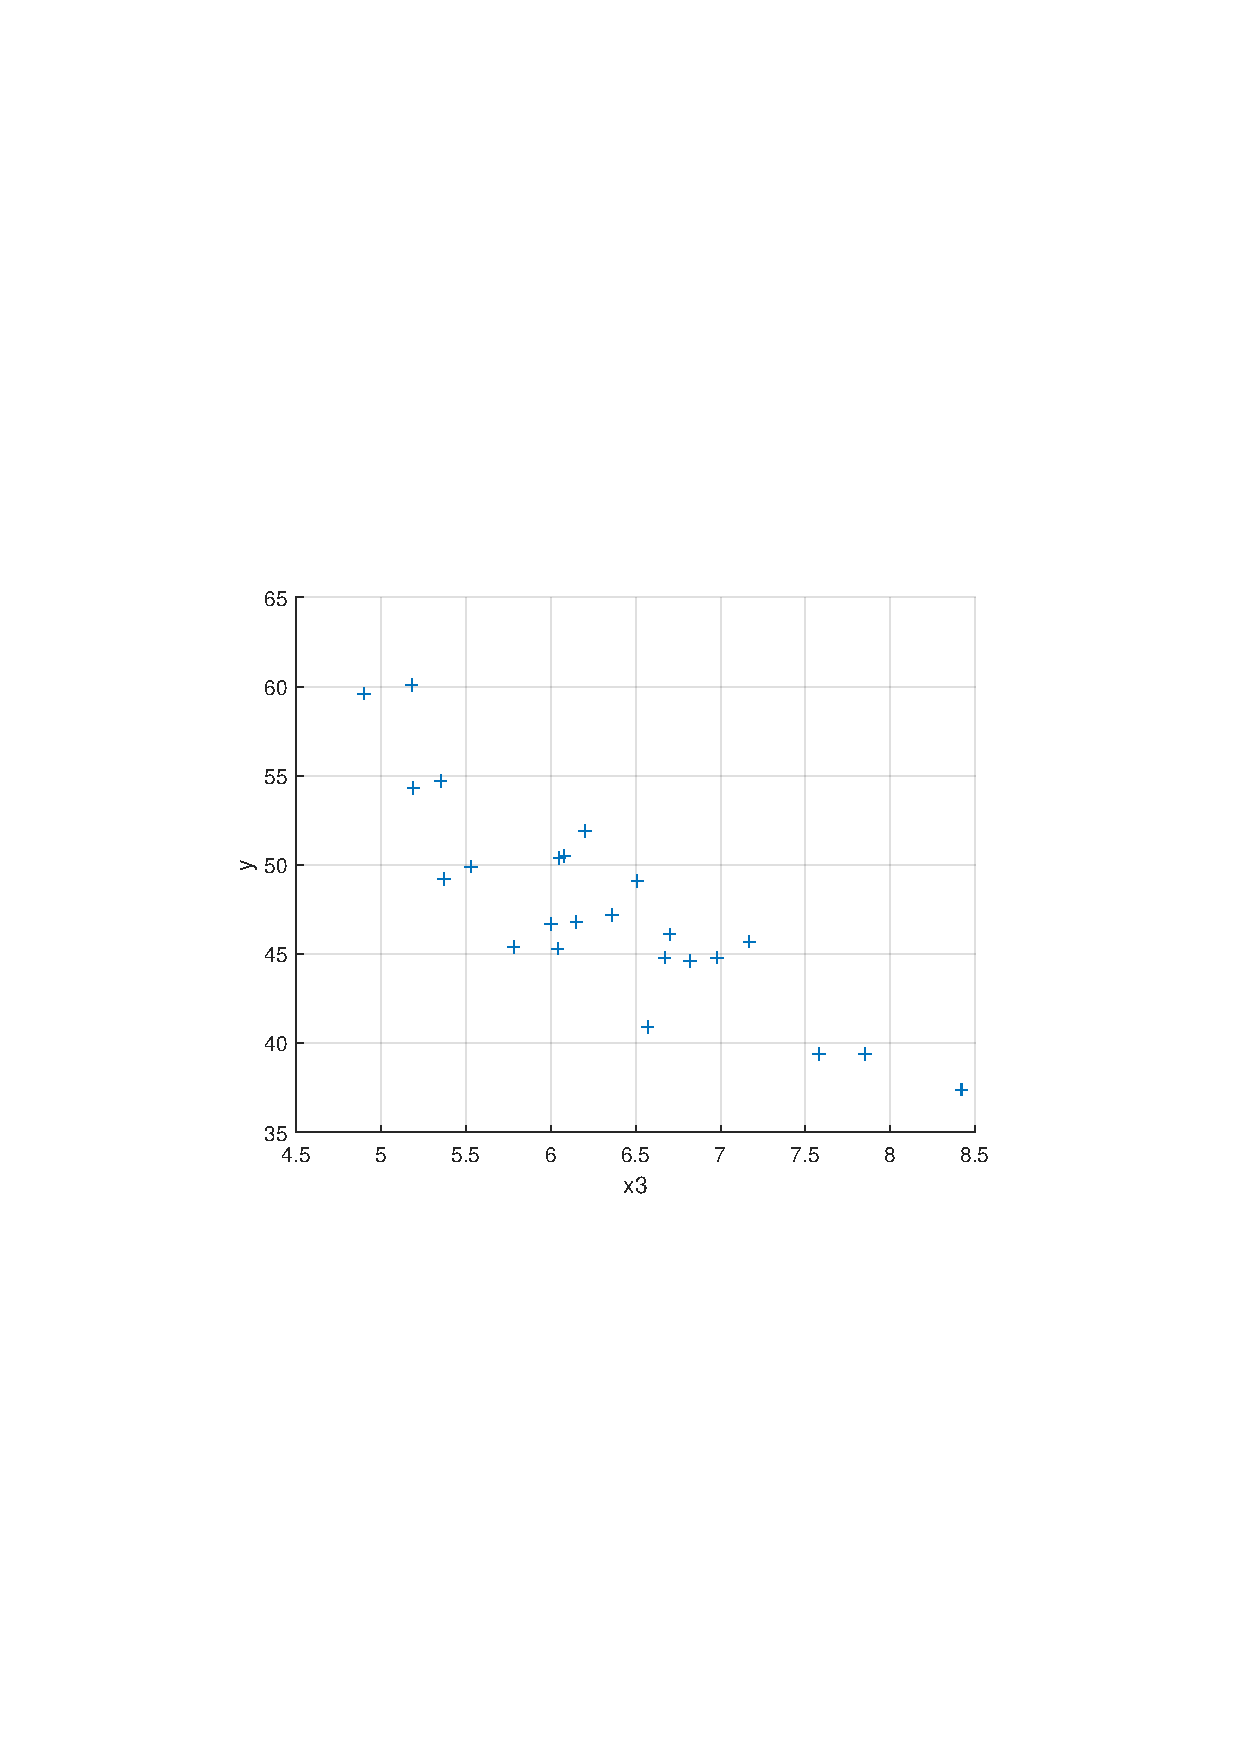
\includegraphics[width=0.3\textwidth,trim={3.09cm 9.295cm 3.09cm 9.295cm},clip]{fig/ex7_scatter_x3.pdf}
    }
    \subfigure[$y$-$x_4$图像]{
        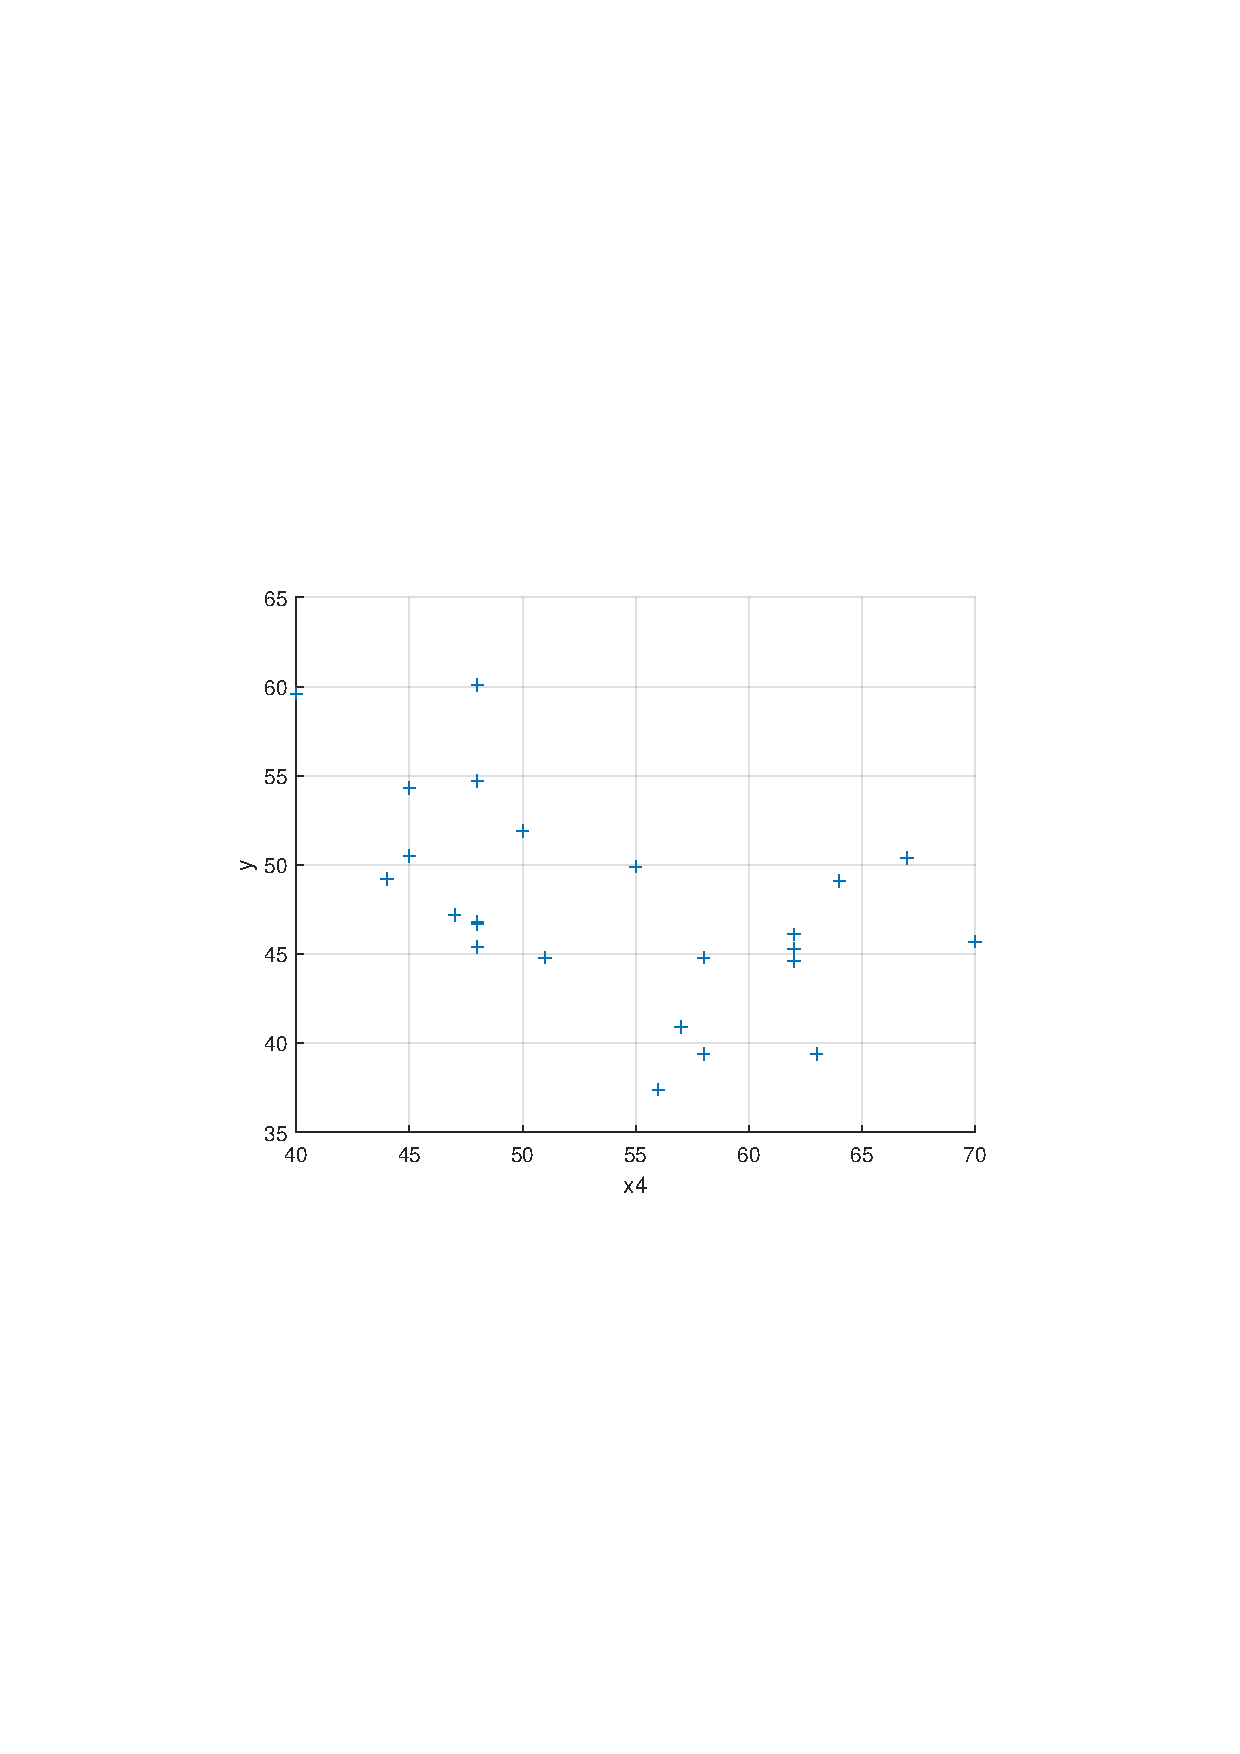
\includegraphics[width=0.3\textwidth,trim={3.09cm 9.295cm 3.09cm 9.295cm},clip]{fig/ex7_scatter_x4.pdf}
    }
    \subfigure[$y$-$x_5$图像]{
        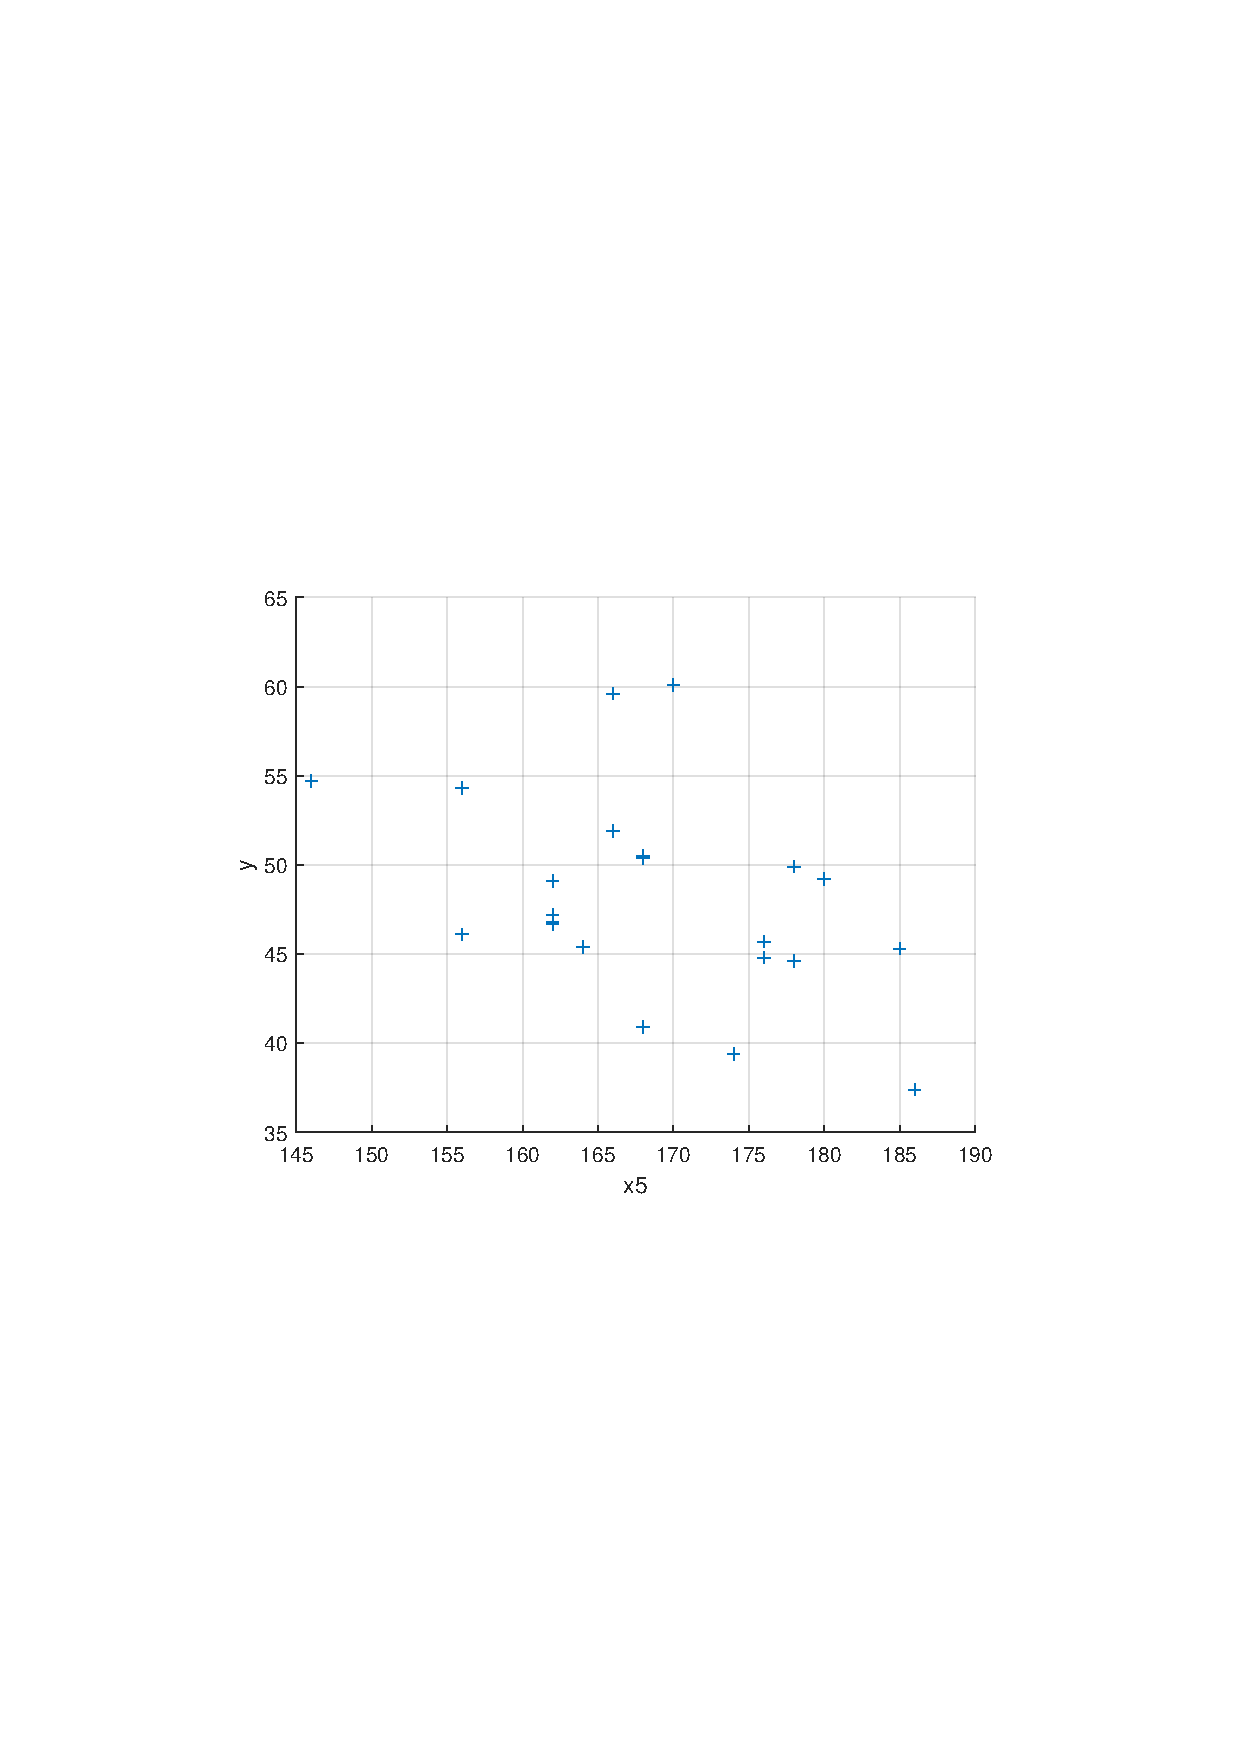
\includegraphics[width=0.3\textwidth,trim={3.09cm 9.295cm 3.09cm 9.295cm},clip]{fig/ex7_scatter_x5.pdf}
    }
    \caption{因变量$y$关于自变量$x_1,x_2,x_3,x_4,x_5$的散点图像}
    \label{fig:ex7_scatter}
\end{figure}

\paragraph{第(2)问:二元回归} 对于二元回归,考虑到高次项的贡献较低,而交叉项不具有明确的实际意义,因此只进行多元线性回归,
\begin{equation}
    y = \beta_0 + \beta_1 x_i + \beta_2 x_j + \varepsilon
\end{equation}

其中$i,j \in \{1,2,3,4,5\}$且规定$i < j$,遍历$i,j$所有的组合,共$C_5^2 = 10$组,对每组$i,j$进行多元线性回归,选出剩余方差$s^2$最小的一组,作为最优的二元回归模型。

在MATLAB中,可使用\texttt{stepwise}命令进行逐步回归,使用\texttt{regress}命令进行最终计算。

\paragraph{第(3)问:多元回归} 对于多元回归,仍然采用多元线性回归的方式,
\begin{equation}
    y = \beta_0 + \sum_{i=1}^5 \beta_i x_i + \varepsilon
\end{equation}

在MATLAB中,同样采用\texttt{stepwise}进行逐步回归的探索,使用\texttt{regress}命令进行多元线性回归的计算。

\paragraph{第(4)问:去除异常点} 残差的置信区间不含零点,则为异常点。在MATLAB中,可通过\texttt{rcoplot}画出残差图,异常点将被标记为红色,然后逐步剔除异常点即可。

\subsubsection{程序}

请参见附录\ref{sec:ex7_code}。

\subsubsection{计算结果}

\paragraph{第(1)问:一元回归} 经过回归分析,计算结果如\Cref{tab:ex7_regress_single},可以看出,在默认的显著性水平$\alpha=0.05$下,选择$x_3,x_4,x_5$时均满足$p<\alpha$,可得到有效的回归模型,其中,当选择$x_3$时,决定系数$R^2$最大,$p$值最小,因此应当选择$x_3$作为自变量,
\begin{equation}\label{eq:ex7_single_best}
    y = 83.44 - 5.67 x_3 + \varepsilon
\end{equation}

\Cref{eq:ex7_single_best}即为最优的一元线性回归模型,此时画出拟合图像和残差图像如\Cref{fig:ex7_single_linear}。

\begin{table}[H]
    \centering
    \caption{一元线性回归模型}
    \label{tab:ex7_regress_single}
    \begin{tabular}{c|ccccccc}
        \toprule
        自变量 & \(\hat{\beta}_0\) & \(\hat{\beta}_1\) & \(\beta_1\)置信区间 & \(R^2\) &
        \(F\) & \(p\) & \(s^2\)\tabularnewline
        \midrule
        \(x_1\) & 64.38 & -0.36 & [-0.83, 0.11] & 0.1025 & 2.5115 & 0.1273 &
        31.2484\tabularnewline
        \(x_2\) & 52.80 & -0.07 & [-0.43, 0.30] & 0.0060 & 0.1337 & 0.7181 &
        34.6053\tabularnewline
        \(x_3\) & 83.44 & -5.67 & [-7.13, -4.21] & 0.7474 & 65.0959 & 0.0000
        & 8.7943\tabularnewline
        \(x_4\) & 67.11 & -0.36 & [-0.63, -0.09] & 0.2631 & 7.8560 & 0.0104 &
        25.6547\tabularnewline
        \(x_5\) & 94.00 & -0.27 & [-0.51, -0.04] & 0.2091 & 5.8169 & 0.0247 &
        27.5352\tabularnewline
        \bottomrule
    \end{tabular}
\end{table}

\begin{figure}[H]
    \centering
    \subfigure[线性拟合]{
        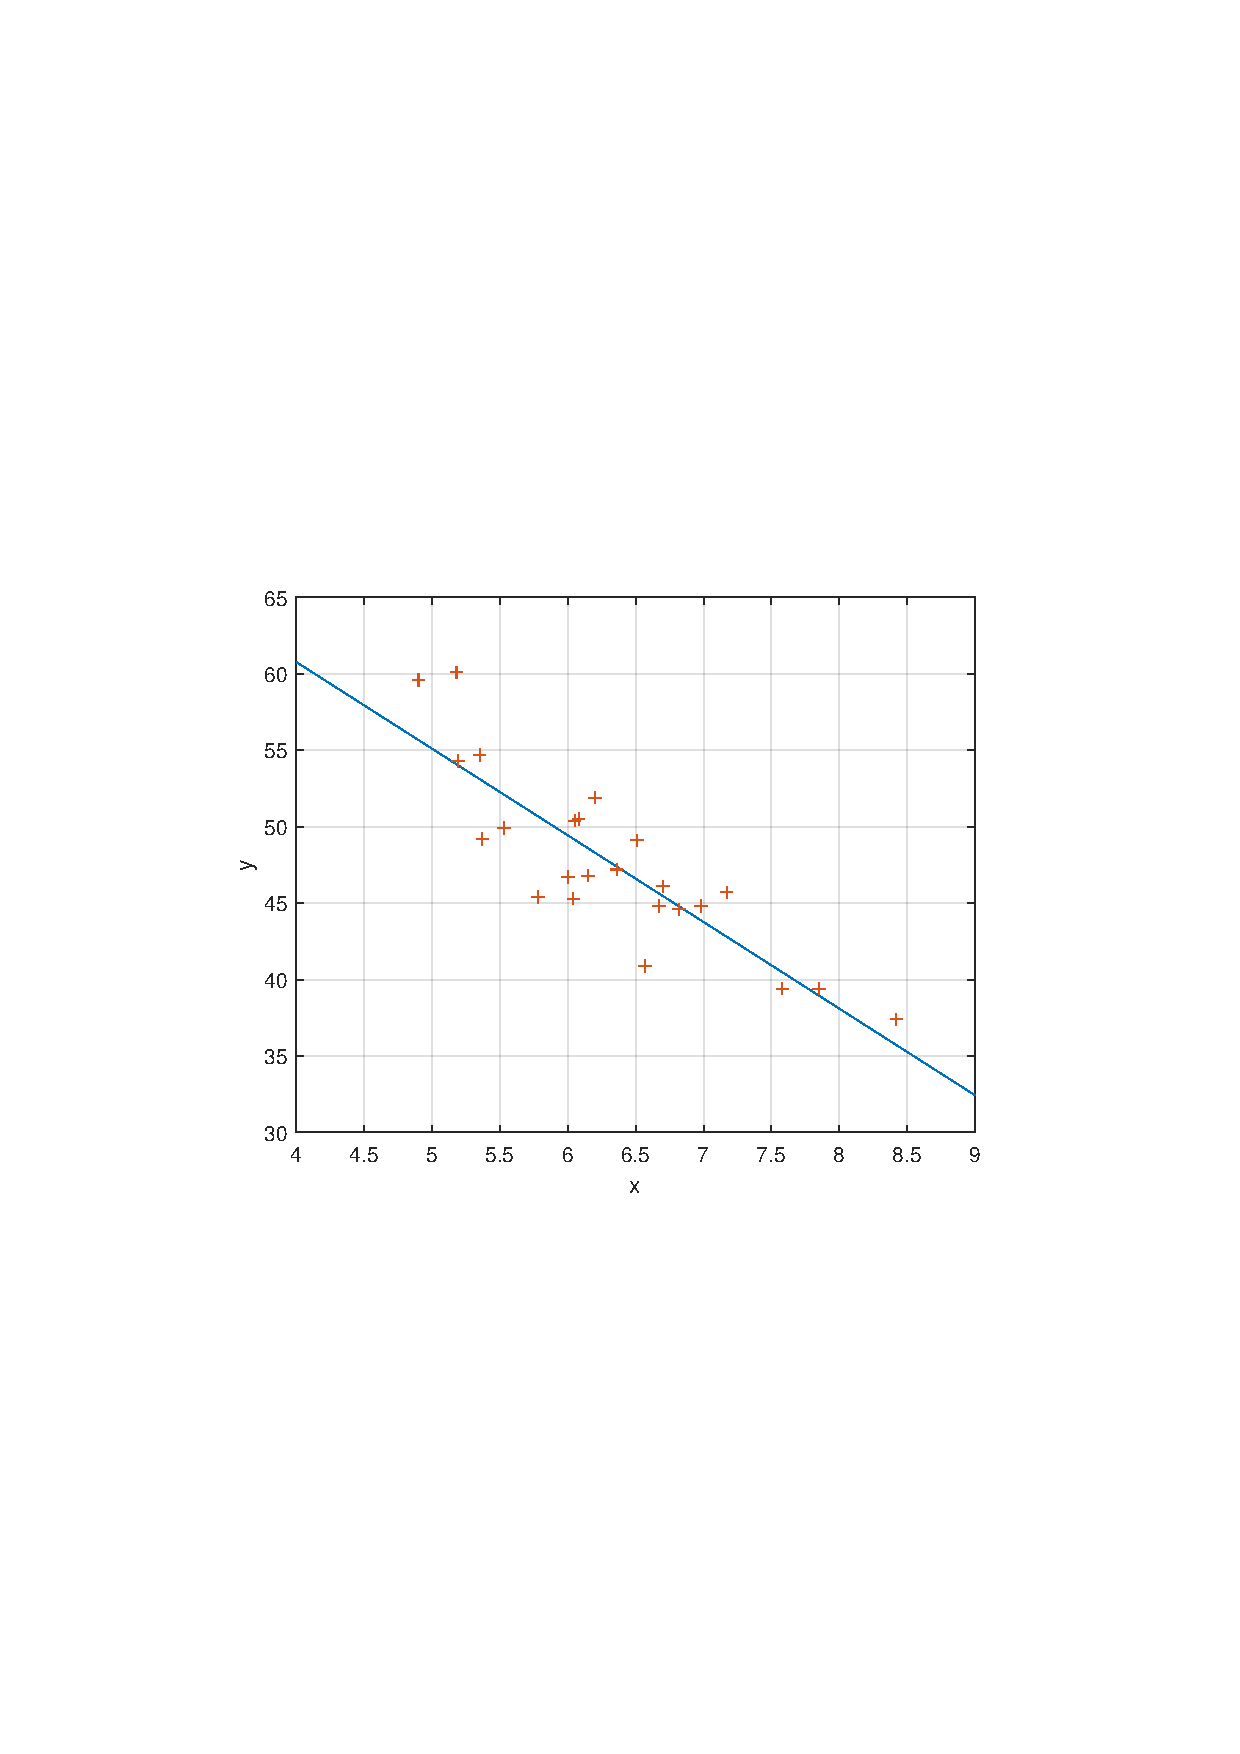
\includegraphics[width=0.47\textwidth,trim={3.09cm 9.295cm 3.09cm 9.295cm},clip]{fig/ex7_single_linear.pdf}
    }
    \subfigure[残差图像]{
        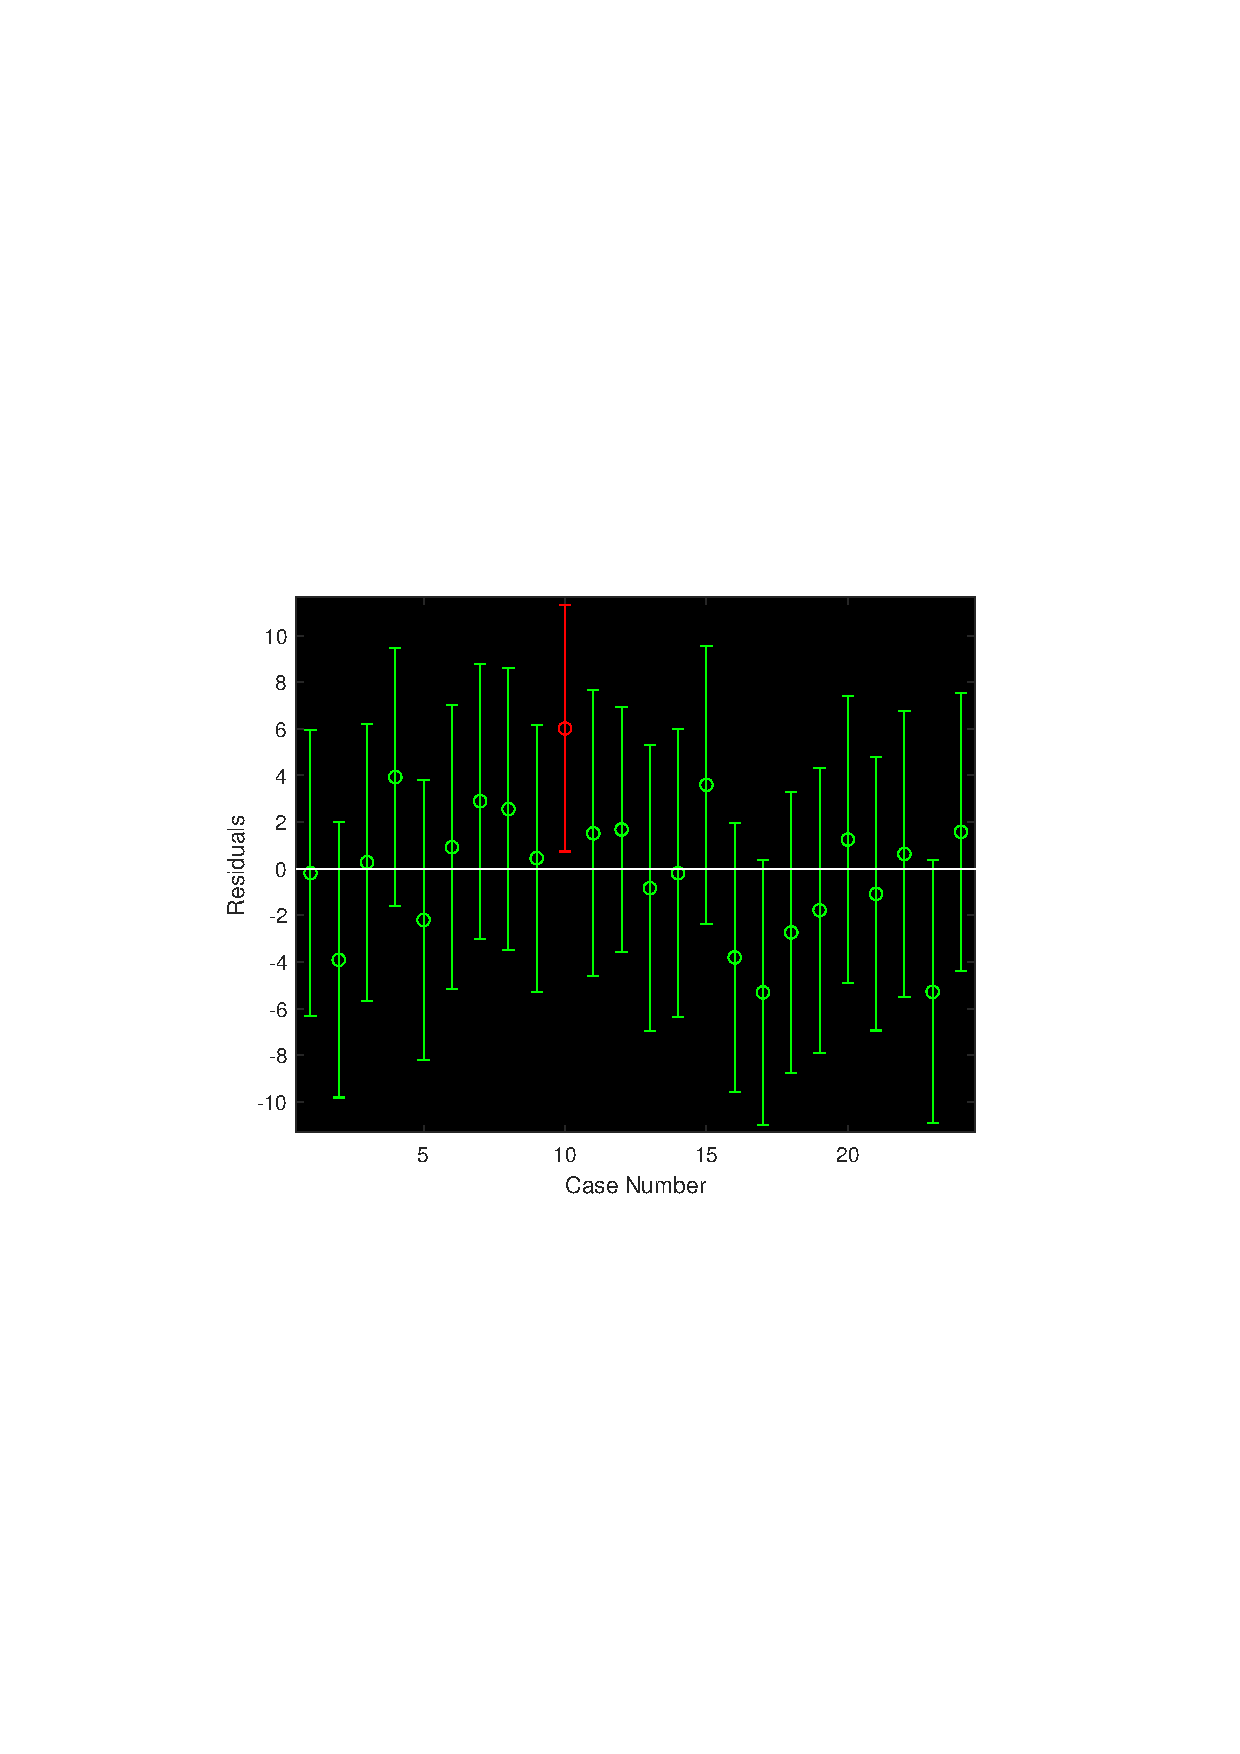
\includegraphics[width=0.47\textwidth,trim={3.09cm 9.295cm 3.09cm 9.295cm},clip]{fig/ex7_single_rcoplot.pdf}
    }
    \caption{一元最优线性回归模型}
    \label{fig:ex7_single_linear}
\end{figure}

为了进一步探索高次回归模型,尝试对自变量$x_3$进行2次和3次多项式回归,得到各回归系数的置信区间如\Cref{tab:ex7_single_poly}。可以看出,当采用2次或3次多项式回归时,最高项系数的置信区间均包含零点,不是有效的回归模型。因此,线性回归模型\Cref{eq:ex7_single_best}即为最优的一元回归模型。

\begin{table}[H]
    \centering
    \caption{一元多项式回归模型}
    \label{tab:ex7_single_poly}
    \begin{tabular}{c|cccc}
        \toprule
        回归模型 & \(\beta_0\)置信区间 & \(\beta_1\)置信区间 &
        \(\beta_2\)置信区间 & \(\beta_3\)置信区间\tabularnewline
        \midrule
        一次多项式 & [74.16, 92.72] & [-7.13, -4.21] & / &
        /\tabularnewline
        二次多项式 & [67.19, 178.26] & [-35.04, -0.78] & [-0.37, 2.24]
        & /\tabularnewline
        三次多项式 & [11.62, 803.26] & [-334.88, 33.02] &
        [-6.79, 49.47] & [-2.44, 0.39]\tabularnewline
        \bottomrule
    \end{tabular}
\end{table}

\paragraph{第(2)问:二元回归} 经过逐步回归和最终计算,得到剩余方差$s^2$最小的二元线性回归模型为,
\begin{equation}\label{eq:ex7_double_best}
    y = 90.85 -0.19 x_1 -5.47 x_3 + \varepsilon
\end{equation}

\Cref{eq:ex7_double_best}即为最优的二元回归模型。详细参数如\Cref{tab:ex7_double_linear},可以看出,回归系数$\beta_1$的置信区间包含零点,表明$x_1$的引入对模型的拟合效果贡献不大。

\begin{table}[H]
    \centering
    \caption{二元线性回归模型}
    \label{tab:ex7_double_linear}
    \begin{tabular}{|c|c|c|}
        \hline
        回归系数 & 估计值 & 置信区间\\
        \hline
        \hline
        \(\beta_0\) & 90.8529 & [77.5587, 104.1471]\\
        \hline
        \(\beta_1\) & -0.1870 & [-0.4337, 0.0598]\\
        \hline
        \(\beta_2\) & -5.4671 & [-6.9059, -4.0283]\\
        \hline
        \multicolumn{3}{|c|}{$R^2=0.7741, \quad F=35.9833, \quad p=0.0000, \quad s^2=8.2389$}\\
        \hline
    \end{tabular}
\end{table}

\paragraph{第(3)问:多元回归} 经过逐步回归和最终计算,得到剩余方差$s^2$最小的多元线性回归模型为,
\begin{equation}\label{eq:ex7_multi_best}
    y = 118.01 -0.33 x_1 -4.57 x_3 -0.16 x_5 + \varepsilon
\end{equation}

\Cref{eq:ex7_multi_best}即为最优的多元回归模型。详细参数如\Cref{tab:ex7_multi_linear}。

\begin{table}[H]
    \centering
    \caption{多元线性回归模型}
    \label{tab:ex7_multi_linear}
    \begin{tabular}{|c|c|c|}
        \hline
        回归系数 & 估计值 & 置信区间\\
        \hline
        \hline
        \(\beta_0\) & 118.0135 & [88.1010, 147.9260]\\
        \hline
        \(\beta_1\) & -0.3254 & [-0.5940, -0.0568]\\
        \hline
        \(\beta_3\) & -4.5694 & [-6.1842, -2.9546]\\
        \hline
        \(\beta_5\) & -0.1561 & [-0.3126, 0.0004]\\
        \hline
        \multicolumn{3}{|c|}{$R^2=0.8143, \quad F=29.2364, \quad p=0.0000, \quad s^2=7.1112$}\\
        \hline
    \end{tabular}
\end{table}

在一元回归、二元回归和多元回归的模型中,多元回归模型\Cref{eq:ex7_multi_best}的剩余方差$s^2$最小,决定系数$R^2$最大,因此将其作为最终模型。

\paragraph{第(4)问:去除异常点} 对最终模型\Cref{eq:ex7_multi_best}进行回归时,画出残差图如\Cref{fig:ex7_outlier_before},其中有两个异常点,去除后又产生了新的异常点,逐步去除所有异常点,序号为4,10,15,17,23,得到的残差图如\Cref{fig:ex7_outlier_after}。

\begin{figure}[H]
    \centering
    \subfigure[去除前]{
        \label{fig:ex7_outlier_before}
        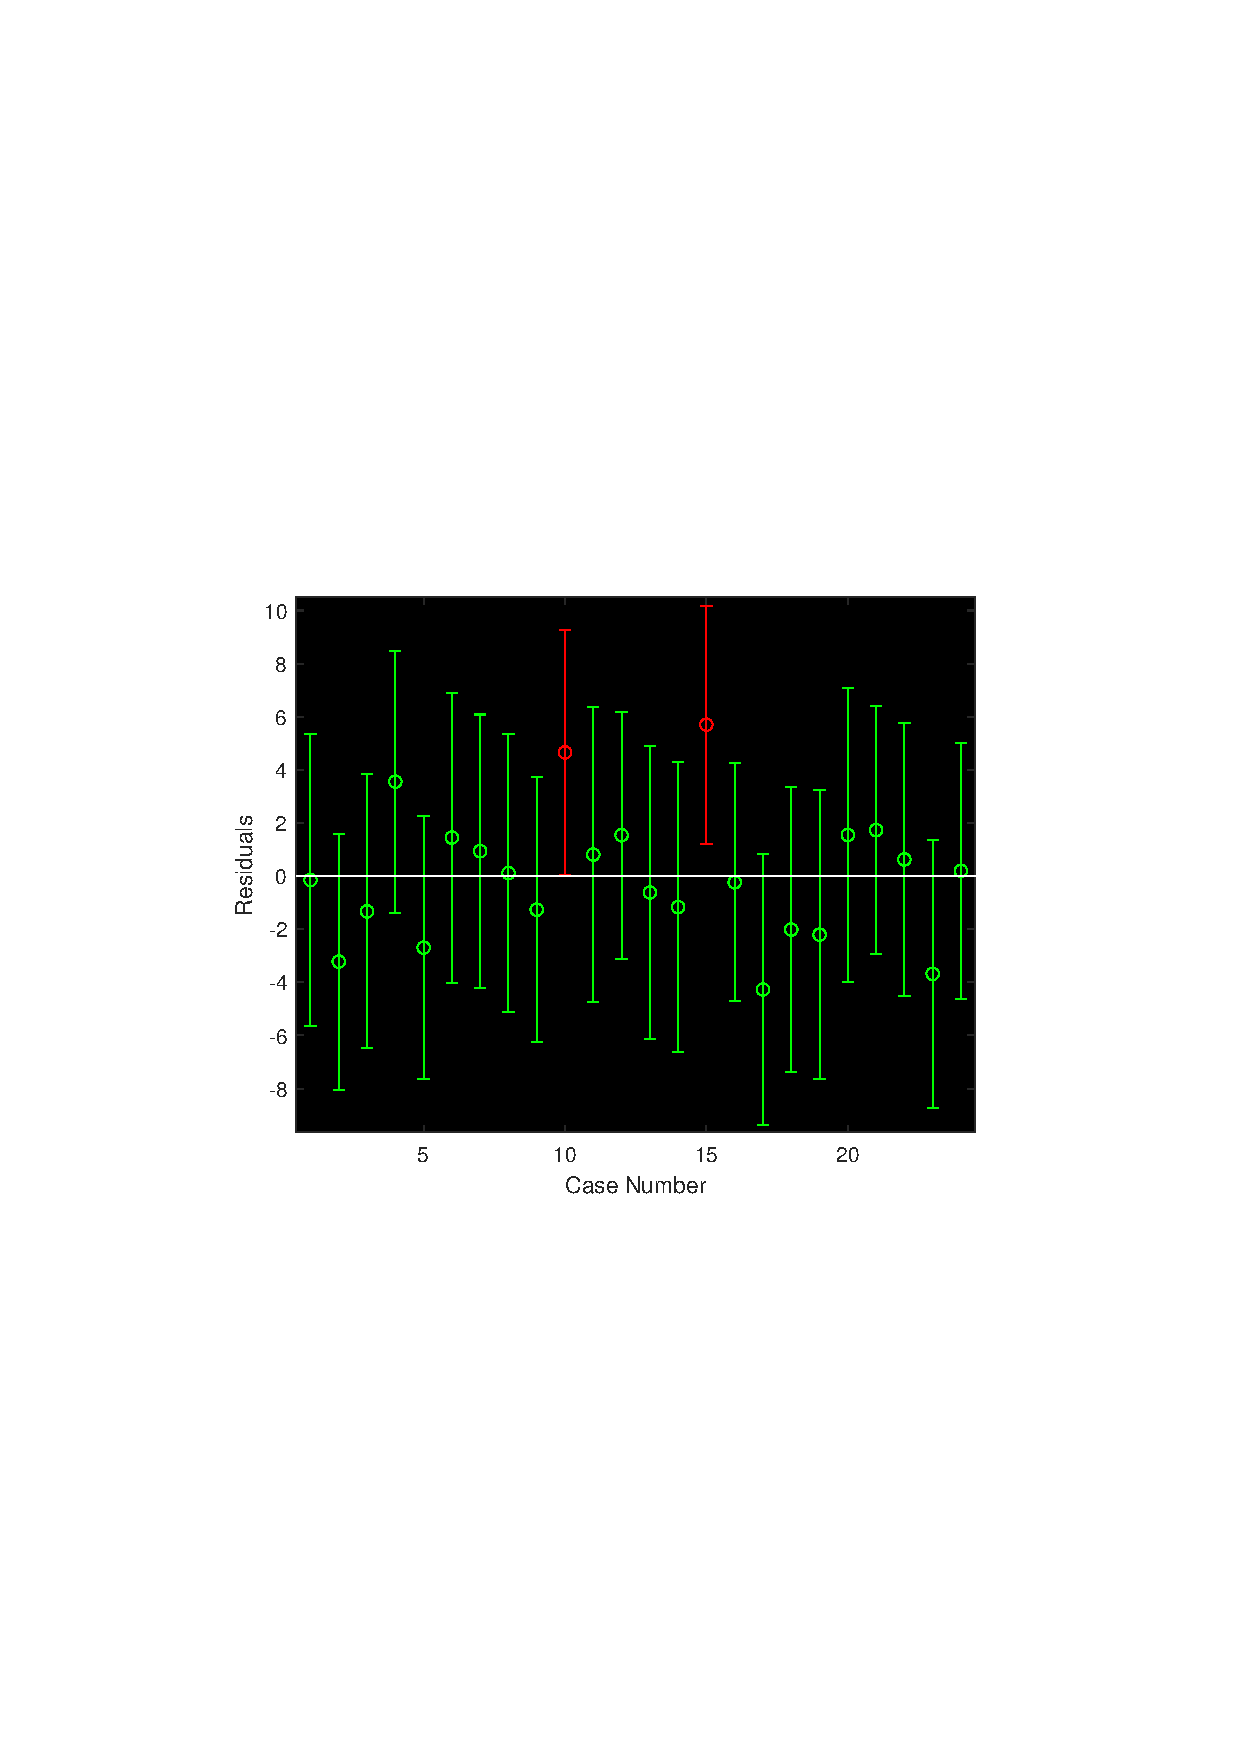
\includegraphics[width=0.46\textwidth,trim={3.09cm 9.295cm 3.09cm 9.295cm},clip]{fig/ex7_outlier.pdf}
    }
    \subfigure[去除后]{
        \label{fig:ex7_outlier_after}
        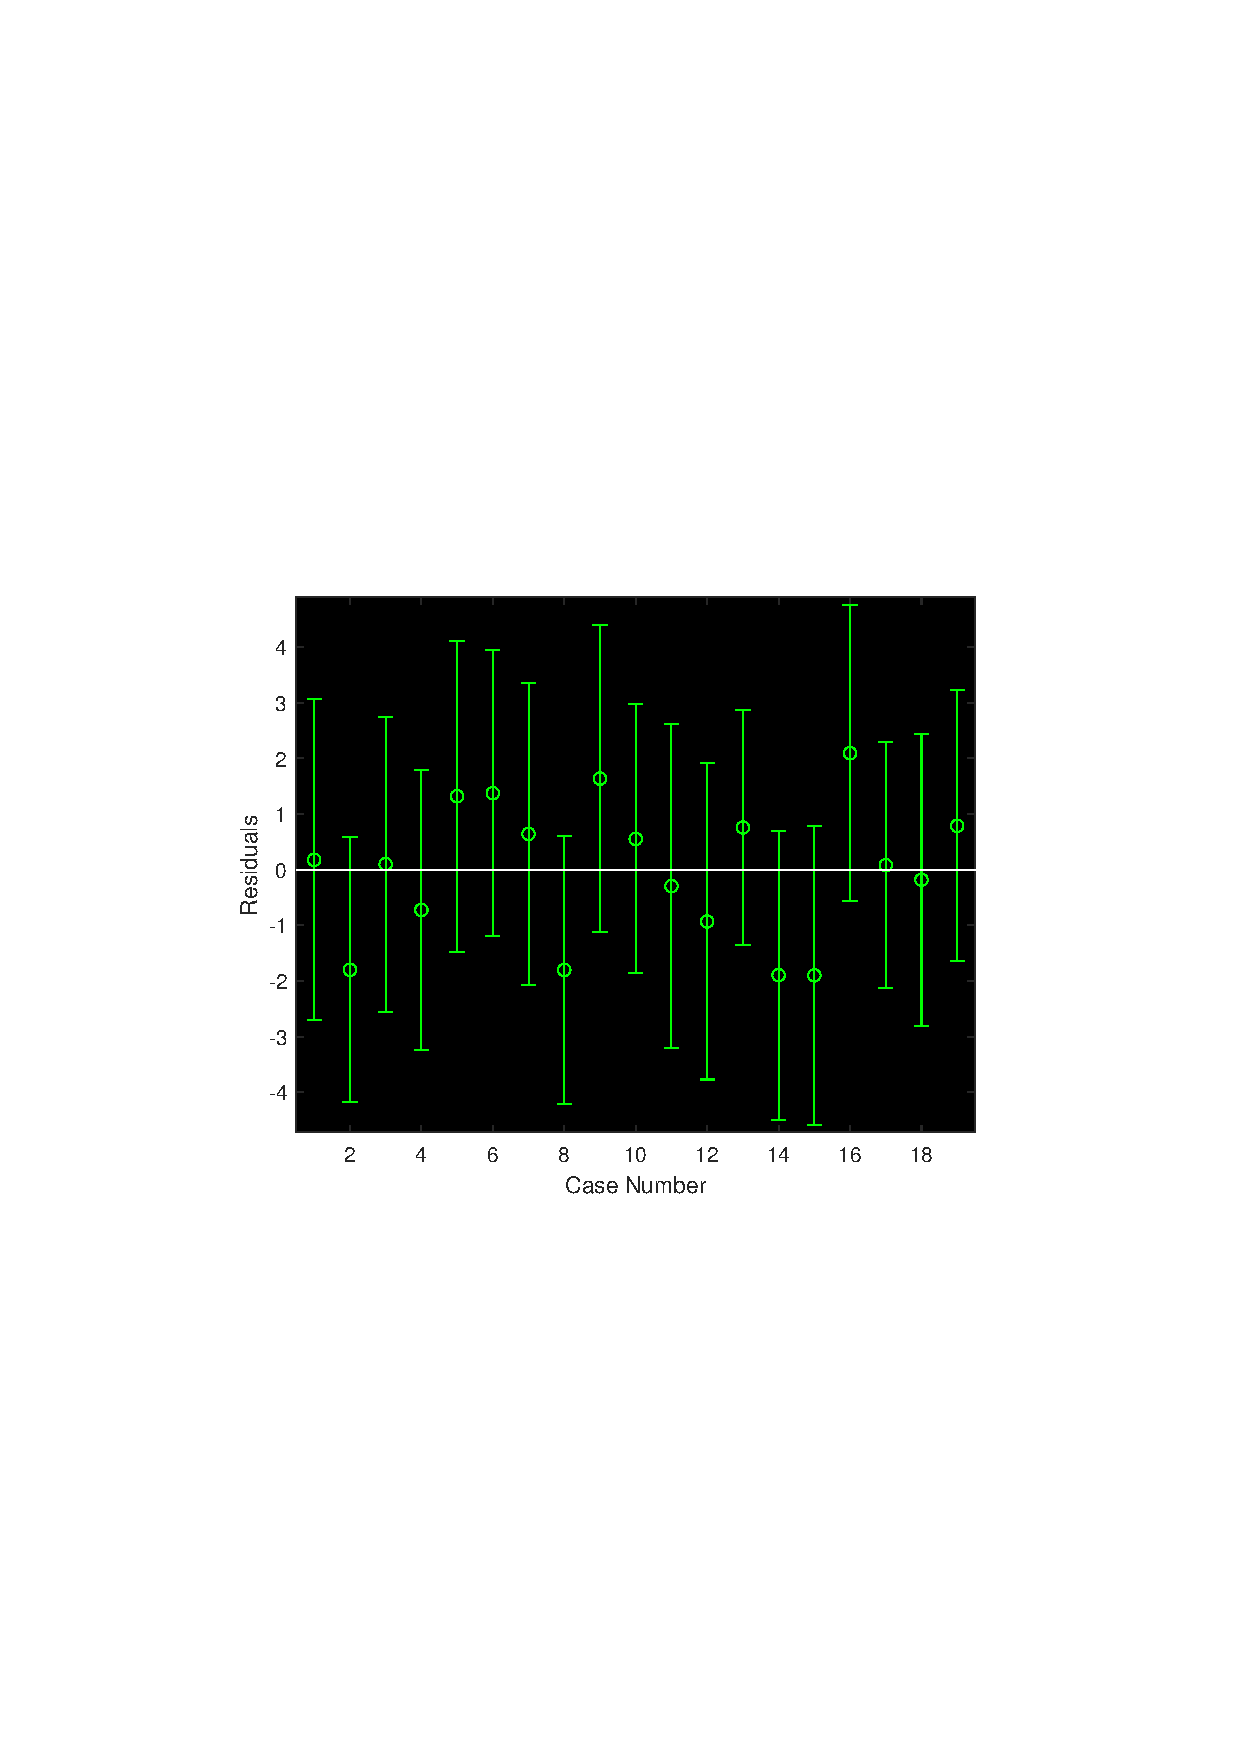
\includegraphics[width=0.46\textwidth,trim={3.09cm 9.295cm 3.09cm 9.295cm},clip]{fig/ex7_outlier_removed.pdf}
    }
    \caption{去除异常点前后的残差图}
    \label{fig:ex7_outlier}
\end{figure}

去除异常点后,模型参数也有了相应的改变,修正后的模型为,
\begin{equation}\label{eq:ex7_final_no_outlier}
    y = 109.35 -0.22 x_1 -3.77 x_3 -0.17 x_5 + \varepsilon
\end{equation}

详细参数如\Cref{tab:ex7_final_no_outlier}。可以看出,去除异常点后,决定系数$R^2$和剩余方差$s^2$都有了明显的改善。

\begin{table}[H]
    \centering
    \caption{去除异常点后的最终模型}
    \label{tab:ex7_final_no_outlier}
    \begin{tabular}{|c|c|c|}
        \hline
        回归系数 & 估计值 & 置信区间\\
        \hline
        \hline
        \(\beta_0\) & 109.3470 & [92.5520, 126.1419]\\
        \hline
        \(\beta_1\) & -0.2230 & [-0.3912, -0.0548]\\
        \hline
        \(\beta_3\) & -3.7694 & [-4.7072, -2.8316]\\
        \hline
        \(\beta_5\) & -0.1652 & [-0.2483, -0.0821]\\
        \hline
        \multicolumn{3}{|c|}{$R^2=0.9268, \quad F=63.3391, \quad p=0.0000, \quad s^2=1.8553$}\\
        \hline
    \end{tabular}
\end{table}

\subsubsection{结果分析}

从最终模型\Cref{eq:ex7_final_no_outlier}可以看出,耗氧能力$y$与年龄$x_1$、1500米跑用时$x_3$、以及跑步后心速$x_5$均呈负相关,即年龄越大、1500米跑得越慢、跑步后心速越快的人,耗氧能力越低,该结论与生活经验相符。

\subsubsection{结论}

若$x_1 \sim x_5$中只许选择1个变量,最好的模型是\Cref{eq:ex7_single_best}。

若$x_1 \sim x_5$中只许选择2个变量,最好的模型是\Cref{eq:ex7_double_best}。

若不限制变量个数,最好的模型是\Cref{eq:ex7_multi_best}。选择\Cref{eq:ex7_multi_best}作为最终模型,因为该模型的剩余方差最小。

最终模型的残差图如\Cref{fig:ex7_outlier_before},共有5个异常点,剔除所有异常点后,模型修正为\Cref{eq:ex7_final_no_outlier}。
